\subsection{%
  Теорема Менгера.%
}

\begin{definition}
  \(uv\)-отделяющее множество это множество вершин, которые необходимо удалить,
  чтобы между \(u\) и \(v\) не было пути.
\end{definition}

\begin{definition}
  \(uv\)-разделяющее множество это множество ребер, которые необходимо удалить,
  чтобы между \(u\) и \(v\) не было пути.
\end{definition}

\begin{theorem}
  Для любой пары несмежных вершин \(u\) и \(v\) в неориентированном графе
  максимальное число внутренне вершинно-независимых путей из \(u\) в \(v\) равно
  минимальной мощности \(uv\)-отделяющего множества.
\end{theorem}
\begin{proof}
  В ходе доказательства будем использовать следующие сокращения:
  \begin{itemize}
    \item ВНП \(:=\) внутренне вершинно независимый путь.
    \item ОМ \(:=\) \(uv\)-отделяющее множество минимальной мощности.
  \end{itemize}

  Сразу оговоримся, что если \(u\) и \(v\) несвязны, то мощность ОМ равна нулю
  \(\implies\) теорема верна. Далее будем считать, что \(u\) и \(v\) связны.
  Обозначим \(S = \{ s_{1}, \dotsc, s_{n} \}\)~--- ОМ и
  \(P_{1}, \dotsc, P_{n}\)~--- множество ВНП.

  Индукция по количеству вершин в графе.

  \textbf{База}: \(n = 3\), тогда мощность ОМ равна единице и существует один
  ВНП.

  \textbf{Переход}: пусть утверждение теоремы верно для графов, у которых менее
  \(n\) вершин. Рассмотрим граф с \(n\) вершинами. Возможны три случая:

  \begin{enumerate}
    \item В графе есть вершина \(x\), которая смежная и с \(u\), и с \(v\).

    Для графа без этой вершины будет выполняться предположение индукции. Если же
    добавить эту вершину в граф, то мощность ОМ увеличится на единицу и при этом
    появится еще один ВНП \(u \to x \to v\).

    \begin{figure}[H]
  \centering
  
  \begin{subfigure}[b]{0.4\textwidth}

    \centering
    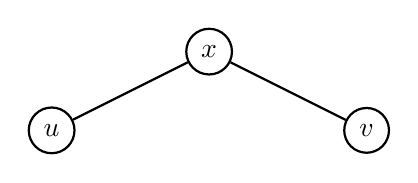
\begin{tikzpicture}[
  point/.style = {
    circle,
    draw = black
  },
  every path/.style = {
    thick
  }
]
  \node[point] (u) at (0, 0) {\(u\)};
  \node[point] (mid) at (2, 1) {\(x\)};
  \node[point] (v) at (4, 0) {\(v\)};

  \draw (u) -- (mid) -- (v);
\end{tikzpicture}

    \caption{1ый случай}

  \end{subfigure}
  \qquad
  \begin{subfigure}[b]{0.4\textwidth}

    \centering
    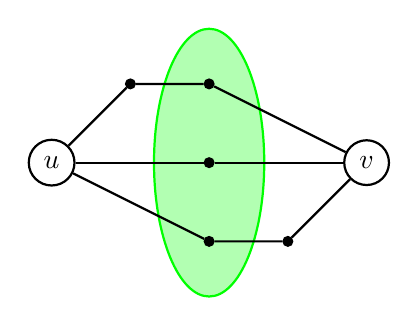
\begin{tikzpicture}[
  dot/.style = {
    shape = circle,
    fill = black,
    minimum size = 4pt,
    inner sep = 0pt,
    outer sep = 0pt,
  },
  point/.style = {
    circle,
    draw = black
  },
  every path/.style = {
    thick
  }
] 
  \draw[draw = green, fill = green!30] (2, 0) ellipse (0.7cm and 1.7cm);
  \node[point] (u) at (0, 0) {\(u\)};
  \node[dot] (p) at (1, 1) {};

  \node[dot] (x) at (2, 1) {};
  \node[dot] (mid) at (2, 0) {};
  \node[dot] (y) at (2, -1) {};

  \node[dot] (q) at (3, -1) {};
  \node[point] (v) at (4, 0) {\(v\)};

  \draw (u) -- (mid) -- (v);
  \draw (u) -- (p) -- (x) -- (v);
  \draw (u) -- (y) -- (q) -- (v);
\end{tikzpicture}

    \caption{2ой случай}

  \end{subfigure}
\end{figure}

    \item Существует ОМ, которое содержит вершину не смежную с \(u\) и вершину,
    не смежную с \(v\).

    Удаление всех вершин из ОМ разобьет его на подграфа \(A\) и \(B\). Из графа
    \(A\) построим граф \(G_{1}\) по следующим правилам:

    \begin{itemize}
      \item Восстановим все вершины из ОМ
      \item Восстановим все ребра, которые соединяли подграф \(A\) и ОМ
      \item Восстановим вершину \(v\)
      \item Добавим ребра из \(v\) в каждую из вершин ОМ
    \end{itemize}

    \begin{figure}[H]
  \centering
  
  \begin{subfigure}[b]{0.4\textwidth}

    \centering
    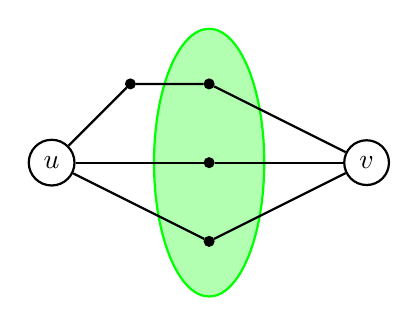
\begin{tikzpicture}[
  dot/.style = {
    shape = circle,
    fill = black,
    minimum size = 4pt,
    inner sep = 0pt,
    outer sep = 0pt,
  },
  point/.style = {
    circle,
    draw = black
  },
  every path/.style = {
    thick
  }
] 
  \draw[draw = green, fill = green!30] (2, 0) ellipse (0.7cm and 1.7cm);
  \node[point] (u) at (0, 0) {\(u\)};
  \node[dot] (p) at (1, 1) {};

  \node[dot] (x) at (2, 1) {};
  \node[dot] (mid) at (2, 0) {};
  \node[dot] (y) at (2, -1) {};

  \node[point] (v) at (4, 0) {\(v\)};

  \draw (u) -- (mid) -- (v);
  \draw (u) -- (p) -- (x) -- (v);
  \draw (u) -- (y) -- (v);
\end{tikzpicture}

    \caption{Граф \(G_{1}\)}

  \end{subfigure}
  \qquad
  \begin{subfigure}[b]{0.4\textwidth}

    \centering
    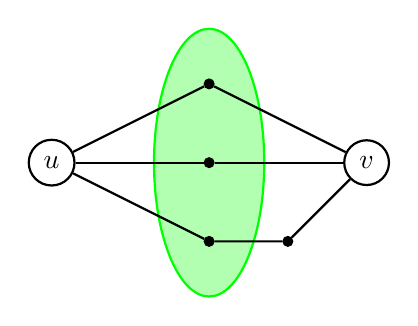
\begin{tikzpicture}[
  dot/.style = {
    shape = circle,
    fill = black,
    minimum size = 4pt,
    inner sep = 0pt,
    outer sep = 0pt,
  },
  point/.style = {
    circle,
    draw = black
  },
  every path/.style = {
    thick
  }
] 
  \draw[draw = green, fill = green!30] (2, 0) ellipse (0.7cm and 1.7cm);
  \node[point] (u) at (0, 0) {\(u\)};

  \node[dot] (x) at (2, 1) {};
  \node[dot] (mid) at (2, 0) {};
  \node[dot] (y) at (2, -1) {};

  \node[dot] (q) at (3, -1) {};
  \node[point] (v) at (4, 0) {\(v\)};

  \draw (u) -- (mid) -- (v);
  \draw (u) -- (x) -- (v);
  \draw (u) -- (y) -- (q) -- (v);
\end{tikzpicture}

    \caption{Граф \(G_{2}\)}

  \end{subfigure}
\end{figure}

    Т.к. по условиям пункта в ОМ существовала вершина, не смежная с \(v\), то в
    полученном графе \(G_{1}\) будет меньше вершин, чем в изначальном. Применив
    к нему предположение индукции получим \(k\) ВНП (по количеству вершин в ОМ)
    вида \(u \leadsto s_{i} \to v\).

    Аналогично из подграфа \(B\) можно построить граф \(G_{2}\) и найти в нем
    \(k\) ВНП вида \(u \to s_{i} \leadsto v\). Из двух полученных множеств путей
    очевидным образом составим искомые ВНП вида \(u \leadsto s_{i} \leadsto v\).

    \item В любой ОМ все вершины смежны с \(u\) и не смежны с \(v\) или
    наоборот.

    \begin{figure}[H]
  \centering

  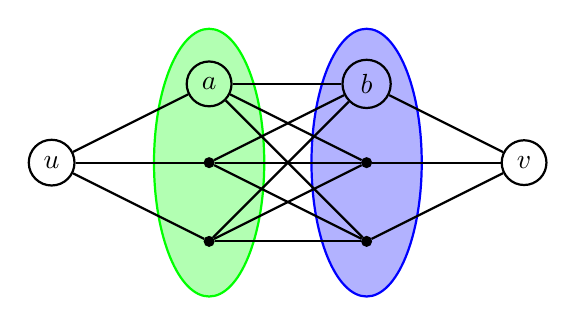
\begin{tikzpicture}[
    dot/.style = {
      shape = circle,
      fill = black,
      minimum size = 4pt,
      inner sep = 0pt,
      outer sep = 0pt,
    },
    point/.style = {
      circle,
      draw = black
    },
    every path/.style = {
      thick
    }
  ] 
    \draw[draw = green, fill = green!30] (2, 0) ellipse (0.7cm and 1.7cm);
    \draw[draw = blue, fill = blue!30] (4, 0) ellipse (0.7cm and 1.7cm);
  
    \node[point] (u) at (0, 0) {\(u\)};
    \node[point] (v) at (6, 0) {\(v\)};
  
    \node[point] (l1) at (2, 1) {\(a\)};
    \node[dot] (l2) at (2, 0) {};
    \node[dot] (l3) at (2, -1) {};
  
    \node[point] (r1) at (4, 1) {\(b\)};
    \node[dot] (r2) at (4, 0) {};
    \node[dot] (r3) at (4, -1) {};
    
    \foreach \idx in {1, 2, 3} {
      \draw (u) -- (l\idx);
      \draw (l\idx) edge (r1) edge (r2) edge (r3);
      \draw (r\idx) -- (v);
    }
  \end{tikzpicture}  
\end{figure}

    Если какая либо вершина не входит ни в одно ОМ, то её удаление не повлияет
    на количество ВНП. Значит её можно удалить и применить предположение
    индукции, поэтому далее будет считать, что каждая вершина принадлежит
    некоторому ОМ.

    Среди вершин, смежных с \(u\) найдется вершина \(a\), которая будет смежна с
    вершиной \(b \neq u\), причем \(b\) будет не смежна с \(u\). Если \(b\) не
    смежна с \(u\), то она смежна с \(v\) по условиям пункта. Получем путь
    \(u \to a \to b \to v\).
    
    Если удалить вершины \(a\) и \(b\), то к полученному графу будет применимо
    предположение индукции. Возвращая вершины \(a\), \(b\) в граф мы добавляем
    один ВНП \(u \to a \to b \to v\) и увеличиваем мощность ОМ на один (в него
    нужно будет взять либо \(a\), либо \(b\)).
  \end{enumerate}
\end{proof}

\begin{remark}
  Приведенная формулировка и доказательство являются 'вершинной' формой теоремы
  Менгера. Существует также и реберная форма теоремы Менгера: для любой пары
  несмежных вершин \(u\) и \(v\) количество реберно-независимых путей из \(u\) в
  \(v\) равно минимальной мощности \(uv\)-разделяющего множества.
\end{remark}
